To motivate the decisions made in our simplified model, we first perform an initial analysis of our empirical data. We will be focusing on the mean service time as our latent variable $\rz$, which is inversely related to airport capacity, or maximum throughput of arrival and departure events, and work on the timescale of a full day for the granularity of $\rz$ and $\rw$, i.e. we only have a single value for each day. Here, we will be assuming that we have a fully specified model for the $\pld{x\given z;y}$ component, but still need to learn $\pld{z\given w}$, which we will do at the same time as learning the relevant posteriors.

\subsection{Flight Data}
Scheduled and actual flight times are taken from the Bureau of Transportation Statistics (BTS) Reporting Carrier On-Time Performance database \cite{bts_transstats_nodate}. Flights from the years 2018 and 2019 are used for training, but analysis is focused on July 2019. Specifically, for each flight in a day, we take the scheduled departure and arrival times for the context $y$, and the actual times for observations $x$, where times are converted to hours past midnight in LGA local time. We restrict our focus to modeling accumulated delays throughout the day, so we do not make additional provisions for cancellations or diversions.

Later, in \cref{sec:atrds-theory}, we will also need to use a coarser encoding of $x$ and $y$ on the same timescale as $z$ and $w$. For this, we will define our aggregation for $x$ as the straight average across all flights in the day, where flights that arrive early are considered as having zero delay instead of negative delay. We will aggregate $y$ by counting the number of operations scheduled in each hour of the day, and taking the maximum, as shown in \cref{fig:split-scheduled-capacity}. We also tried using the total number of flights in the day as a measure of aggregate scheduled demand, and obtained similar results.

\begin{figure}[htb!]
    \centering
    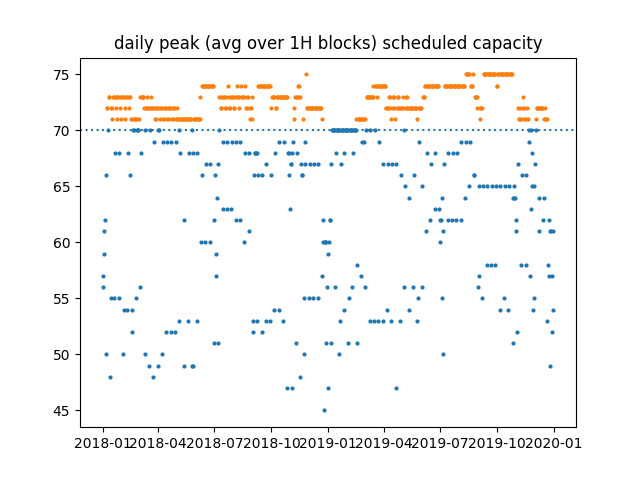
\includegraphics[width=0.8\linewidth]{media/lga-analysis-14.png}
    \caption{Daily peak scheduled hourly demand in 2018 and 2019, in operations per hour.}
    \label{fig:split-scheduled-capacity}
\end{figure}

\subsection{Weather Data}
We restrict our focus to considering the impact of visibility and ceiling, as these weather conditions are known to directly affect airport capacity \cite{2014lga}. Measurements are taken from the National Oceanic and Atmospheric Administration (NOAA) Local Climatological Data Version 2 (LCDv2) dataset \cite{weatherdata}, and converted to the Meteorological Aerodrome Report (METAR) format commonly used in aviation. Specifically, visibility is already given as an hourly value, but ceiling must be inferred from provided sky condition data by taking the height of the lowest cloud layer with at least 4 oktas of coverage.

For our encoding as a daily aggregate value, we use the harmonic mean~\cite{ferger1931nature} for the sky ceiling, to reflect the greater relevance of lower values, and similarly select the daily minimum for the visibility. We clip values at $10000$ feet and $10$ statute miles for ceiling and visibility respectively, for numerical stability, and because there is not really any meaningful difference among higher values.


\subsection{Initial Motivating Analysis}

To see why our choice of variables is well motivated for a proof of concept study, we examine the relationship between weather and delays, which our learned model should be able to reflect, if it is a good representation. First, we note that lower ceilings and visibilities appear to partially coincide with days with higher delays, as shown in \cref{fig:2019-07-weather-delay-timeline}.

\begin{figure}[htb!]
    \centering
    % 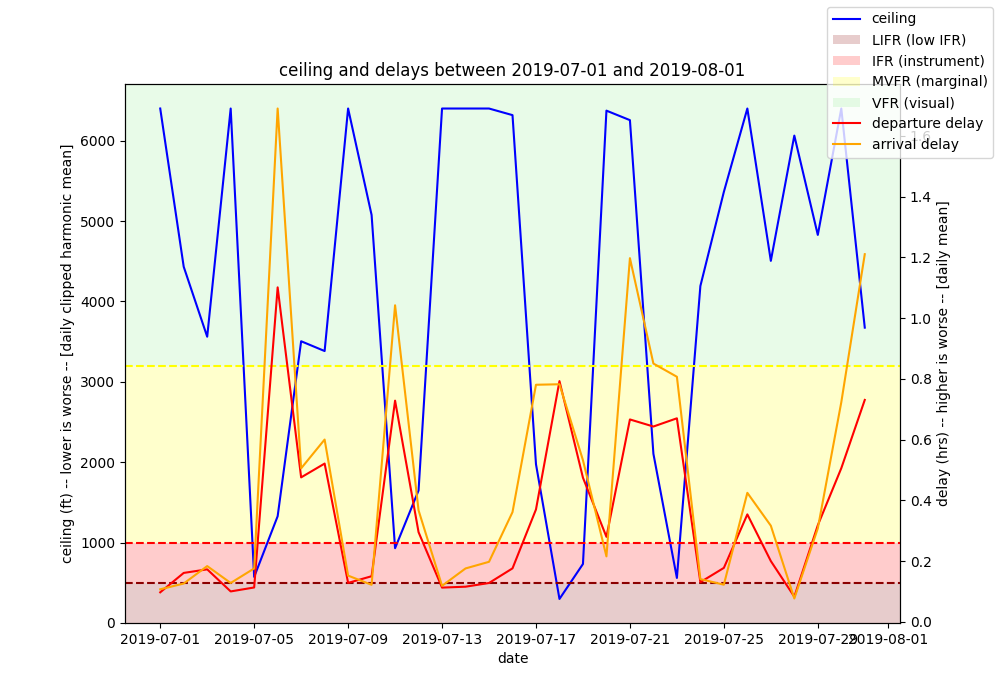
\includegraphics[height=5.5cm]{media/lga-analysis-1.png}
    % 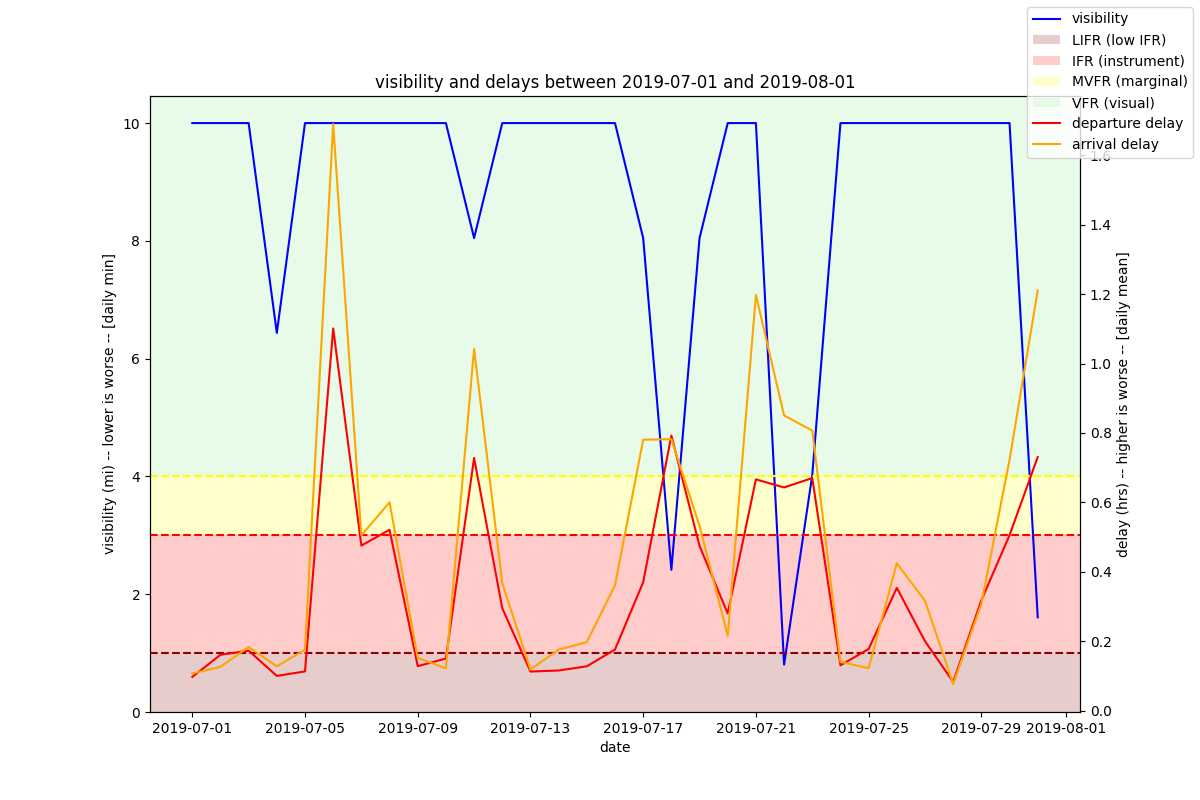
\includegraphics[height=5.5cm]{media/lga-analysis-3.png}
    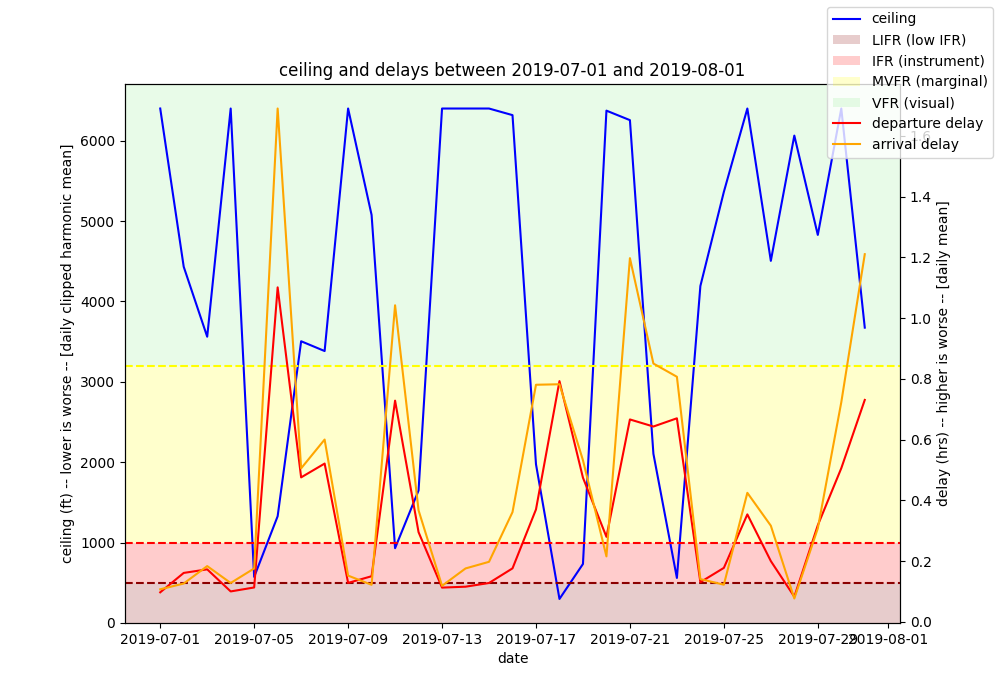
\includegraphics[width=.66\linewidth]{media/lga-analysis-1.png}
    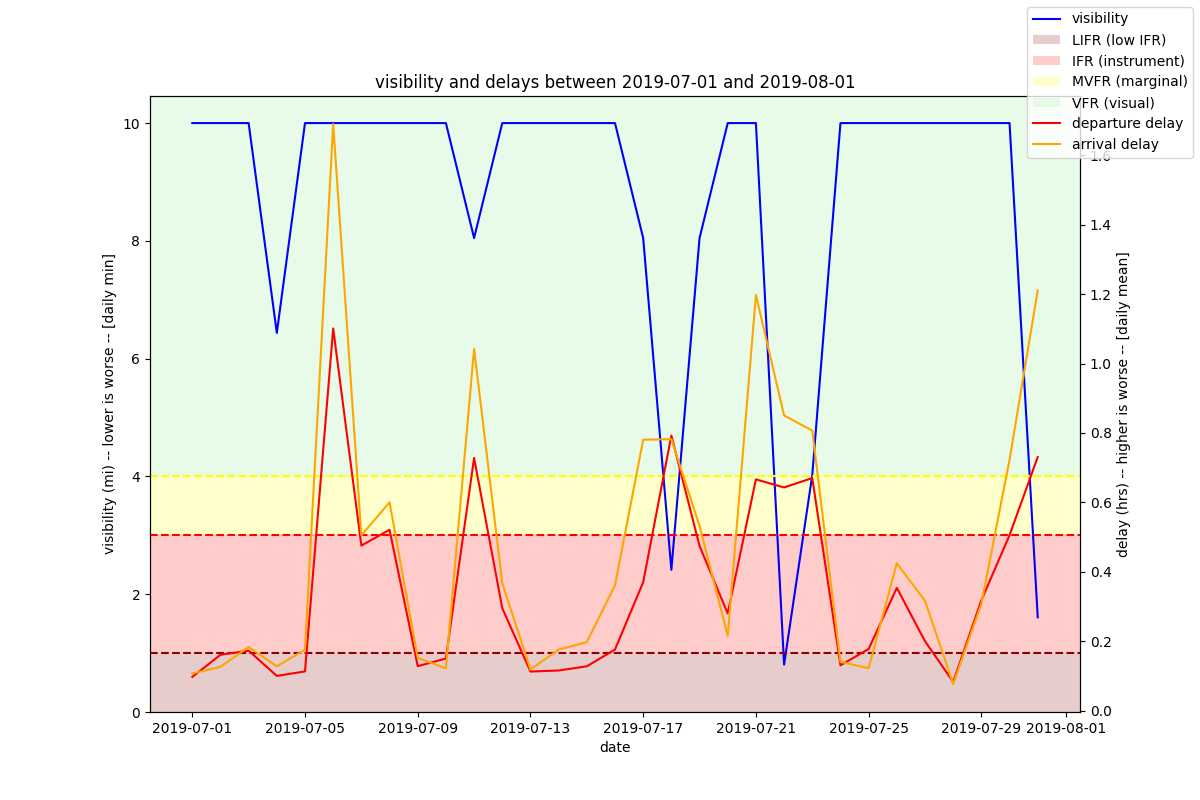
\includegraphics[width=.66\linewidth]{media/lga-analysis-3.png}
    \caption{Timeline of ceiling (upper) and visibility (lower) compared to delays in July 2019. Days with poorer weather, where the blue line is lower, coincide with days with greater delays, where the red and orange lines are higher. Flight rule regions show severity of weather.}
    \label{fig:2019-07-weather-delay-timeline}
\end{figure}

\begin{figure}[htb!]
    \centering
    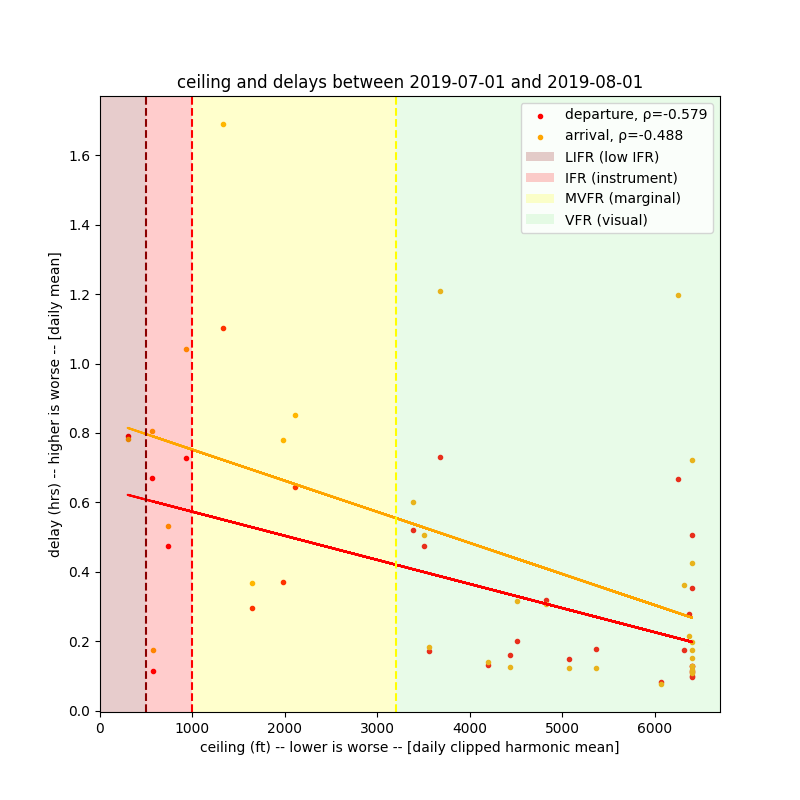
\includegraphics[height=8.1cm]{media/lga-analysis-2.png}
    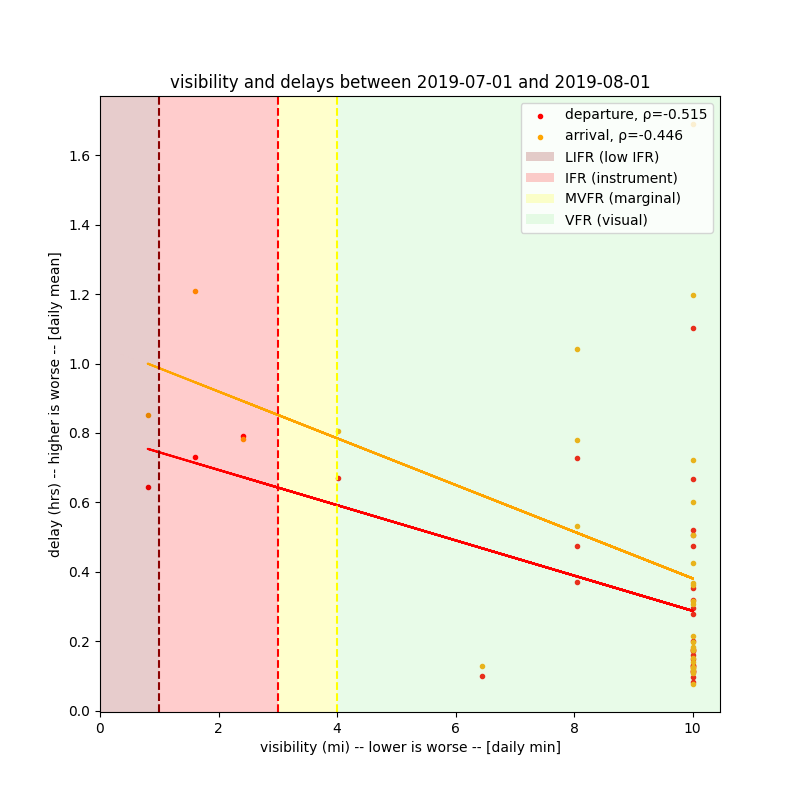
\includegraphics[height=8.1cm]{media/lga-analysis-4.png}
    \caption{Scatter plot of ceiling (left) and visibility (right) compared to delays in July 2019.}
    \label{fig:2019-07-weather-delay-scatter}
\end{figure}

Here, instrument flight rule (IFR) weather conditions are supposed to lead to a lower maximum throughput, meaning likely higher delays, than visual flight rule (VFR) conditions, which appears to align well with what we observe. To make this relationship a bit more obvious, we also show the same data in the timeline as a scatter plot with trend line and Pearson correlation coefficient, in \cref{fig:2019-07-weather-delay-scatter}. 


It is important to re-iterate, however, that weather is not the only factor that is considered in modeling delays, as is emphasized in \cref{fig:bubble3d-all}. We can see that higher scheduled capacity, corresponding to busier days, are more prone to delays at the same weather conditions compared to a lighter day, for example. This distinction in distribution of delays given weather is illustrated in \cref{fig:bubble2d-split}, which is essentially a 2D top view of an upper and lower partition of the full 3D plot.

\begin{figure}[htb!]
    \centering
    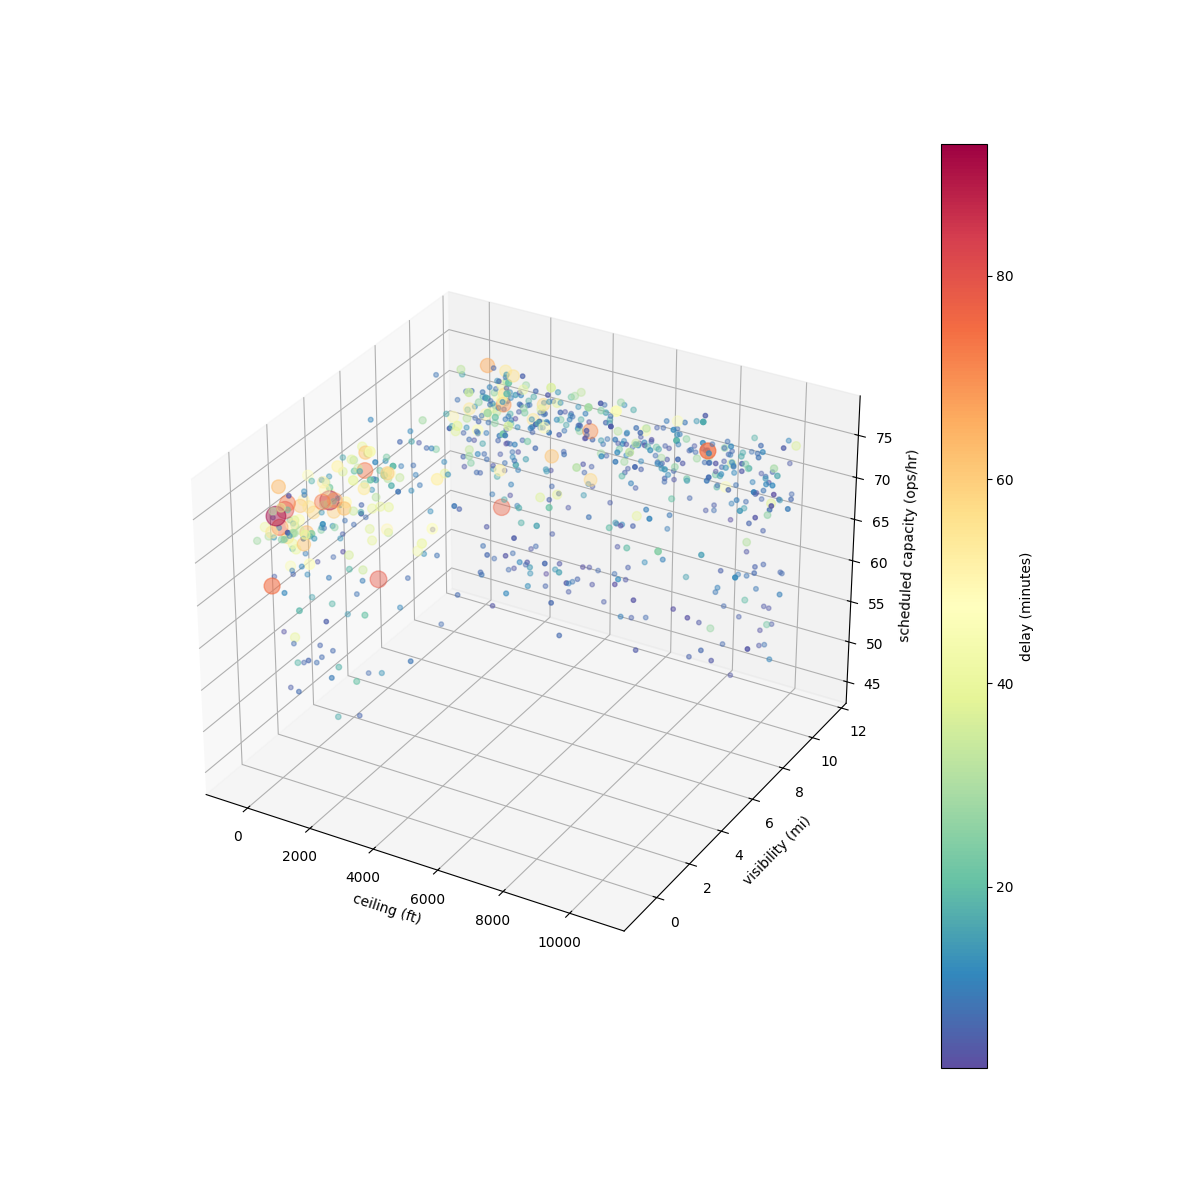
\includegraphics[width=\linewidth]{media/lga-analysis-17.png}
    \caption{3D scatter plot of both weather conditions and scheduled demand for each day in 2018 and 2019, where delay is represented with color. Points with higher delay also have greater size and opacity, for emphasis, and some noise is added for visualization purposes. }
    \label{fig:bubble3d-all}
\end{figure}

\begin{figure}[htb!]
    \centering
    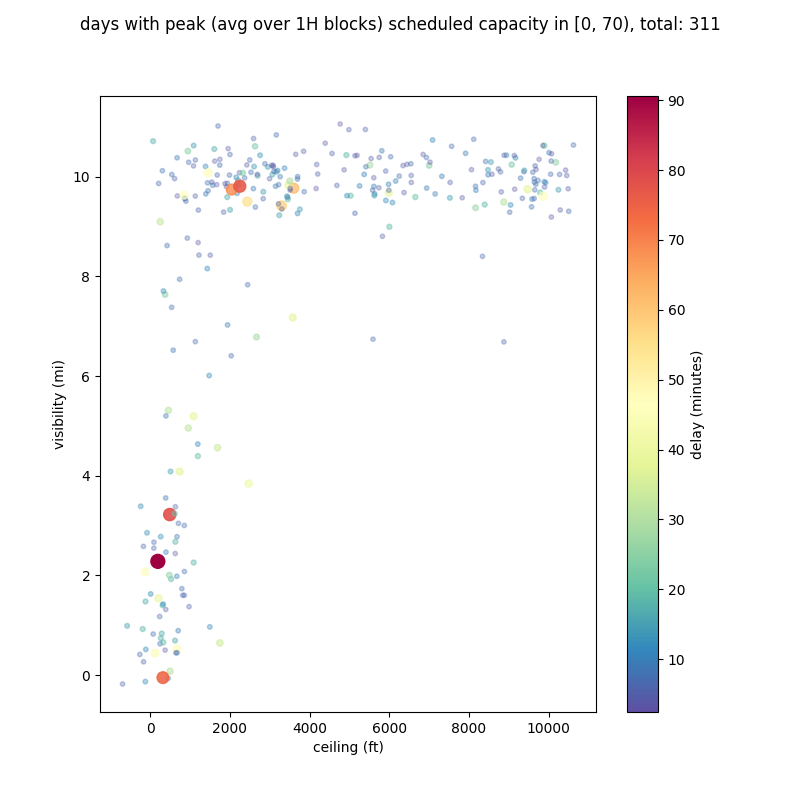
\includegraphics[height=8.0cm]{media/lga-analysis-15.png}
    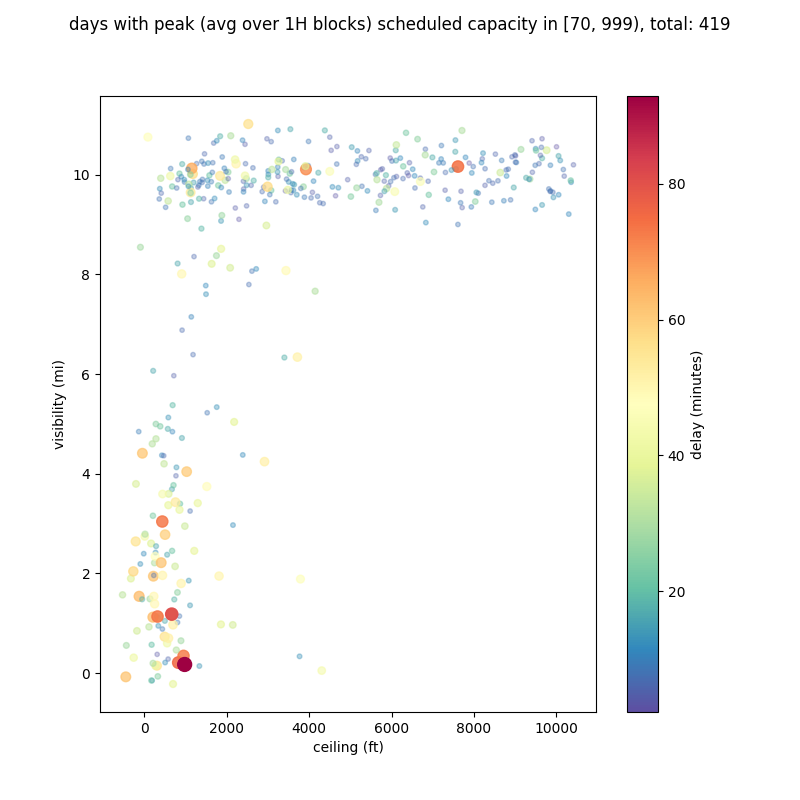
\includegraphics[height=8.0cm]{media/lga-analysis-16.png}
    \caption{Different distributions of delays given weather for lighter (left) and busier (right) days, which shows that failures are more concentrated in the region of higher demand and worse weather.}
    \label{fig:bubble2d-split}
\end{figure}

\subsection{Stochastic Airport Simulation}

We extend and adapt the stochastic queuing model developed in \cite{dawson2024breaking, michael_peng_probing_2024}, which was originally developed to study the mass cancellations and delays during the 2022 Southwest Airlines winter weather crisis, to better support our particular use case of less severe, but still impactful weather conditions. Specifically, we make two main changes.

The first is that we extend the model to be closer to reality, in terms of flights included. The original model only includes flights that have both endpoints, i.e. arrival and departure airport, within the set of 4 to 10 key network airports included. Additionally, only flights operated by Southwest are tracked. We add support for including all airline carriers present in the schedule data simultaneously, and also implement tracking for flights with one endpoint outside of the network. This is done by adding a source supernode, which emits all flights originating from outside the network to the relevant airports, and a sink supernode, to which all flights headed outside of the network are directed. The departure times at which flights are emitted from the source node are considered exogenous variables taken directly from the context, and we support a wide range of options including both scheduled and actual times. For this study, we choose to use the actual times, so that delays that are mainly attributable to LGA are properly modeled, and so that the demand profile of incoming flights when fitting our model is as realistic as possible.

The second change is that we add support for additional types of flight failures. The original simulation models delays and eager cancellations that result from when there are not enough available aircraft at an airport to depart at the scheduled time. We extend this to also model lazy cancellations, where flights that have been waiting to depart for long enough are canceled. Analogously, flights that have been waiting to arrive, which corresponds to waiting in holding patterns, are also considered failed after a given amount of time, because it is unrealistic for flights to wait for arrivals indefinitely. For this proof of concept, however, we disable both of these features, as minimal impact was observed in the very simplified scenario. Similarly, the actions taken, i.e. deciding which flights and when to cancel or delay, is set to the simple default strategy of first in first out (FIFO), but in future work, incorporating choice of strategy into the simulation will be important, as the end goal is stress-testing future design decisions.

With this in mind, our simulation roughly proceeds as follows. Flights are emitted from the source supernode at given times, to represent external incoming demand. The ego airport, which in this case is LGA, also has departing flights it must attempt to accommodate. When flights are ready to depart or arrive at the ego airport, they are entered into a service queue to await processing. We use a single M/M/1 queue for this, where a single server handles all flights regardless of their arrival or departure status. The time between arrivals and departures is drawn from an exponential distribution, where the mean $\lambda^{-1}$ is the latent mean service time parameter. This simulates a Poisson process with rate $\lambda$, which explains the connection between our introduced mean service time and the more commonly seen airport capacity or throughput. Roughly speaking, higher mean service times can lead to increased delays if severe enough, because it will mean that the airport may become unable to handle the demand of scheduled flights and must cancel or delay some in order to operate within its current limits. We also note that this service time is meant to encompass all factors that might affect throughput at a single airport, and not necessarily just the impact from visual versus instrument flight rules.

In this simplified setting, we directly bake in the notion of the action $\ra$ into the simulation, so we make no attempt to learn it implicitly. Similarly, we do not have any learned process parameters $\theta$ that are relevant to $\pld{x\given z;y}$, as we assume that we are working with a fully specified simulator. This is also implemented as a model through Pyro, a probabilistic programming language \cite{bingham2019pyro}, which makes the simulation differentiable, and gives us access to the likelihoods, so that we can use stochastic variational inference methods directly.

It is also important to reiterate here that mean service time on its own is not the only factor relevant to delays. \cref{fig:busy-light-comparison} shows two days that did not have significant delays in reality, after artificially imposing a higher mean service time of $0.2$ hours on both and simulating the result, and observing that the busier day was hit harder. This makes sense intuitively as well, because we would expect it to be easier to recover from a disruption with less external stress, so we can expect lighter days to be more tolerant to higher service times.

\begin{figure}[htb!]
    \centering
    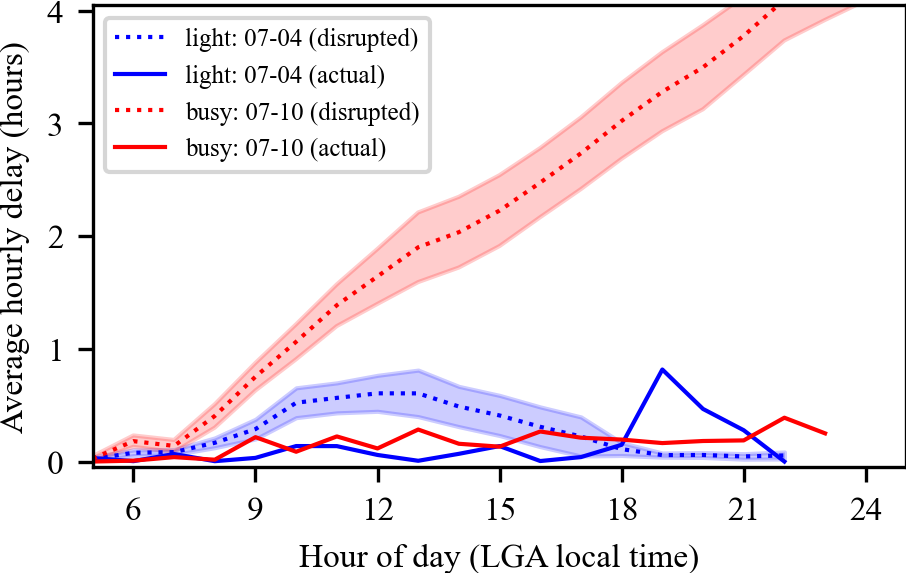
\includegraphics[width=0.7\linewidth]{media/busy_light_comparison.png}
    \caption{Demonstration of the effect of scheduled demand on delays on days with similar actual outcomes (solid lines). The same simulated disruption is applied to two days (dotted lines, shaded is standard deviation), showing that the lighter day (blue) is less affected than the busier (red).}
    \label{fig:busy-light-comparison}
\end{figure}

\subsection{Weather-Informed Priors}

We partially specify a simple mixture density model for the $\pld{z\given w}$ component. Specifically, we define a function $\fvn: w\mapsto c$ parameterized by $\nu$, where $c\in \ms C = \{0,1\}$ represents nominal and failure weather. 
\begin{proposition}[Weather Mixture Density Model]
    Then, we define our model as the following:
    \begin{equation}
        \pld{z\given w} = \begin{cases}
            \mt N(z;\mu_0, \sigma_0^2) \quad \text{if }\fvd{w} = 0\\
            \mt N(z;\mu_1, \sigma_1^2) \quad \text{if }\fvd{w} = 1,
        \end{cases}
    \end{equation}
    where $\mt N(\cdot;\mu,\sigma^2)$ denotes the univariate normal density with mean $\mu$ and variance $\sigma^2$.
\end{proposition}

We judgmentally select $\mu_0 = 0.012$ and $\sigma_0 = 0.001$ for nominal weather, and $\mu_1 = 0.019$ and $\sigma_1 = 0.001$ for failure weather, to incorporate the belief that worse weather leads to higher service times. 

\begin{proposition}[Relaxation of Threshold Classification for $\fvn$]
    For the decision function $\fvn$, we use a simple threshold classification given by
    \begin{align}
        \fvd{w} & = 1 - \sigma\left(\alpha (w_v-\wthvf)\right)\cdot \sigma\left(\alpha (w_c-\wthcf )\right) \\
        &\approx \begin{cases}
            1 \;\; \text{if} \;\; w_v \leq \wthvf \;\; \text{or}\;\;  w_c \leq \wthcf \\
            0 \;\; \text{otherwise}
        \end{cases}
    \end{align}
    where $\sigma(x)=(1+e^{x})^{-1}$ is the sigmoid function, and $\alpha = 50$ is a fixed scaling parameter to control the sharpness of the threshold.
\end{proposition}


Here, we let $w = (w_v, w_c) $, to represent the individual visibility and ceiling components, and let $\nu = (\wthvf,\wthcf)$ be thresholds parameterizing $\fvn$ that must be learned. We can interpret this model as imposing weather-informed priors on $z$ based on $w$, instead of just assuming the same prior for all observations, to incorporate the effect of weather. Additionally, we can extend this to the continuous case $\ms C=[0,1]$ directly by linearly interpolating between the nominal and failure density accordingly, as we will use in \cref{sec:atrds-theory}.

While we chose to specify all $\mu_c$ and $\sigma_c$, we also note that these can be set to different values, to investigate what the learned thresholds might be to decide between various severity levels of service time impact. 